\chapter{Conclusion}
In this thesis a solution to the scalability problem of classical RSA-based group sharing scheme was given with respect to not violate any security requirements \ref{sec:requirements} that where already present in the reference system. Classical systems suffer from many file-keys that need to be maintained each time a new file is updated or a new member joins a group. Existing members need to make sure that the newly joined member can access all previous shared files by decrypting all file-keys and encrypting them again with the new members public key, creating own file keys for the new member. If a new file is updated, it need to made accessable to all members in the group. A file need to be encrypted one by one for each public key in the group. Creating $n$ more file-keys per file upload.

Different approaches are analyzed and argumentatively compared to end-up with an MA-ABE scheme fits the requirements and solves the scalability problem the best.  MA-ABE uses attribute to create an access policy under which a file is secured. This access policy acts like a shared group key that is only accessible to the members that satisfy this access policy. In that way does MA-ABE solves the initial problem of creating $n$ file keys per new file update. Each scheme using a group key only needs to encrypt the file once using the group key resulting in one shared file-key. 

MA-ABE was chosen as the best candidate, because it, in comparison to other secure-group communications, does not redistribute the shared group key to other members. The main feature of an ABE scheme is that the users inherently possesses all needed information to calculate the group key from their given attribute secrets. 

MA-ABE is especially important in the field of applied ABE schemes, since it divides the universe of attributes into different separated clusters, each managed and maintained by an own, self-organized AA. This breaks up a disadvantage of classical ABE schemes: the global decryption power of the system administrator or single AA. 

From the current field of MA-ABE schemes TF-DAC-MACS was the candidate that showed great scalability and performance, no global decryption power of the CA and a mechanism to revoke users from the system. Since it does not support 1-of-n threshold gate policies (OR-gates), an improved version to this scheme, called \name, was constructed and implemented. To further make \name more practically applicable the fix two-factor constrain was made optional. 

To evaluate whether \name indeed scales better than the classical rekeying scheme different benchmarks were performed against a reference implementation of the classical RSA-based rekeying scheme. The outcome was that regarding the number of file-keys \name scales better with a worst-case scenario were \name scales in the same way as the reference implementation. However, it was noticeable that this feature comes with additional overhead in file-key size. Taking this observation into account archives the prototype a better scalability when at most $n/2$ "OR"-gates are used in the access policy. 

Regarding performance a completely different picture is drawn. Due to the assumption that the number of attributes to describe a group is equal or less to the number of users in the group \name shows a better performance since it only works with the attributes and not the users directly. Depending on the underlying system and the chosen distribution of attributes to users an intersecting point can be calculated when \name shows a better performance. This intersecting point is located in the best-case scenario (Figure \ref{fig:1-for-infty-and}) at around 145 users. 

To achieve a better single encryption performance than the classical system at least 145 users need to be describable with one attribute. The resulting implication is that \name benefits from large scale systems with a lot of users that share a lot of attributes. Small groups that share perform peer-to-peer sharing suffer more from the additional overhead. Here \name can only be beneficial if storage and not computing power is the bottleneck. 

\section{Practical Applicability}

\begin{figure}[!ht]
\centering
    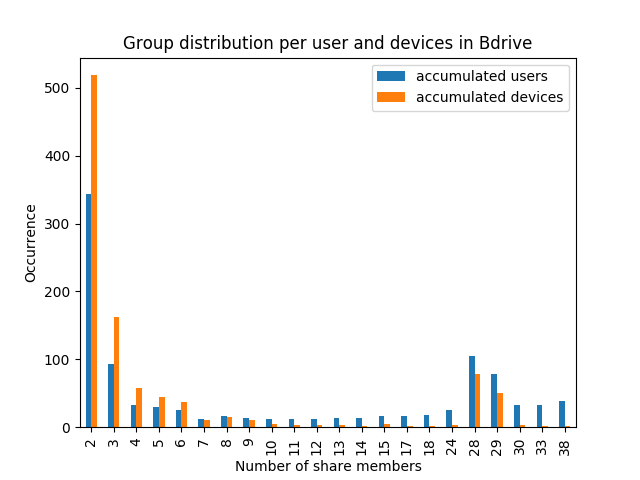
\includegraphics[width=1.0\linewidth]{img/share_distribution_bdirve.png}
    \caption{The distribution of shared folders per users and their aggregated devices.}
    \label{fig:evaluation-share-distribution}
\end{figure}

In the evaluation capture \ref{sec:evaluation} it was concluded that in the best-case scenario \name performs and scales better than the Bdrive from 145 users in a group onwards if they all can be described by the same attribute. To validate that is a common scenario in the real world the distribution of groups and their members of Bdrive are listed in Figure \ref{fig:evaluation-share-distribution}.

As it can be extracted from the figure, many users share file only to one or two other users. In that case would \name provide no performance  advantage. Really interesting for the ABE use case is the second spike at 28 to 30 members. Since Bdrive is addressed to business it can be assumed that this second spike define the company wide shared folders. It can be expected that for very large scale companies that have more then 300 employees. If they all are members in the same share/name can use its full potential, since all members will share a common attribute: "Employee in Company X".

In conclusion \name can reduce the number of file-keys dramatically if combined with the right access policy. It depends on the company administrator to assign each user suitable attributes so that fine-grain access formulas without using "OR"-gates can be constructed.  
\section{Future adaptations}

\todo{
* Data owner Id can relate to the selected two factor key. 
* This would enable us to have multible keys 2FA keys per user. each securing an own CT. 
* make ownerId -> 2FA id 

* Handle attributes on device level and not on user level 
}